% This is "sig-alternate.tex" V2.0 May 2012
% This file should be compiled with V2.5 of "sig-alternate.cls" May 2012
%
% This example file demonstrates the use of the 'sig-alternate.cls'
% V2.5 LaTeX2e document class file. It is for those submitting
% articles to ACM Conference Proceedings WHO DO NOT WISH TO
% STRICTLY ADHERE TO THE SIGS (PUBS-BOARD-ENDORSED) STYLE.
% The 'sig-alternate.cls' file will produce a similar-looking,
% albeit, 'tighter' paper resulting in, invariably, fewer pages.
%
% ----------------------------------------------------------------------------------------------------------------
% This .tex file (and associated .cls V2.5) produces:
%       1) The Permission Statement
%       2) The Conference (location) Info information
%       3) The Copyright Line with ACM data
%       4) NO page numbers
%
% as against the acm_proc_article-sp.cls file which
% DOES NOT produce 1) thru' 3) above.
%
% Using 'sig-alternate.cls' you have control, however, from within
% the source .tex file, over both the CopyrightYear
% (defaulted to 200X) and the ACM Copyright Data
% (defaulted to X-XXXXX-XX-X/XX/XX).
% e.g.
% \CopyrightYear{2007} will cause 2007 to appear in the copyright line.
% \crdata{0-12345-67-8/90/12} will cause 0-12345-67-8/90/12 to appear in the copyright line.
%
% ---------------------------------------------------------------------------------------------------------------
% This .tex source is an example which *does* use
% the .bib file (from which the .bbl file % is produced).
% REMEMBER HOWEVER: After having produced the .bbl file,
% and prior to final submission, you *NEED* to 'insert'
% your .bbl file into your source .tex file so as to provide
% ONE 'self-contained' source file.
%
% ================= IF YOU HAVE QUESTIONS =======================
% Questions regarding the SIGS styles, SIGS policies and
% procedures, Conferences etc. should be sent to
% Adrienne Griscti (griscti@acm.org)
%
% Technical questions _only_ to
% Gerald Murray (murray@hq.acm.org)
% ===============================================================
%
% For tracking purposes - this is V2.0 - May 2012

\documentclass{acm_proc_article-sp}

\usepackage{graphicx}
\usepackage{caption}
\usepackage{subcaption}
\usepackage{url}

% Redefines \@ptsize to make setspace happy
% \makeatletter
% \renewcommand{\@ptsize}{0}
% \makeatother

% Double-spaces the entire document
%\usepackage{setspace}
%\doublespacing

\begin{document}
%
% --- Author Metadata here ---
\conferenceinfo{WOODSTOCK}{'97 El Paso, Texas USA}
%\CopyrightYear{2007} % Allows default copyright year (20XX) to be over-ridden - IF NEED BE.
%\crdata{0-12345-67-8/90/01}  % Allows default copyright data (0-89791-88-6/97/05) to be over-ridden - IF NEED BE.
% --- End of Author Metadata ---

\title{Recognition of Continuous Gestures with Dynamic Hand Pose and Path for
Mid-Air Interaction}
%
% You need the command \numberofauthors to handle the 'placement
% and alignment' of the authors beneath the title.
%
% For aesthetic reasons, we recommend 'three authors at a time'
% i.e. three 'name/affiliation blocks' be placed beneath the title.
%
% NOTE: You are NOT restricted in how many 'rows' of
% "name/affiliations" may appear. We just ask that you restrict
% the number of 'columns' to three.
%
% Because of the available 'opening page real-estate'
% we ask you to refrain from putting more than six authors
% (two rows with three columns) beneath the article title.
% More than six makes the first-page appear very cluttered indeed.
%
% Use the \alignauthor commands to handle the names
% and affiliations for an 'aesthetic maximum' of six authors.
% Add names, affiliations, addresses for
% the seventh etc. author(s) as the argument for the
% \additionalauthors command.
% These 'additional authors' will be output/set for you
% without further effort on your part as the last section in
% the body of your article BEFORE References or any Appendices.

\numberofauthors{2} %  in this sample file, there are a *total*
% of EIGHT authors. SIX appear on the 'first-page' (for formatting
% reasons) and the remaining two appear in the \additionalauthors section.
%
\author{
% You can go ahead and credit any number of authors here,
% e.g. one 'row of three' or two rows (consisting of one row of three
% and a second row of one, two or three).
%
% The command \alignauthor (no curly braces needed) should
% precede each author name, affiliation/snail-mail address and
% e-mail address. Additionally, tag each line of
% affiliation/address with \affaddr, and tag the
% e-mail address with \email.
%
% 1st. author
\alignauthor
% Ying Yin\\
%        \affaddr{Massachusetts Institute of Technology}\\
%        \affaddr{}\\
%        \affaddr{}\\
%        \email{yingyin@csail.mit.edu}
% 2nd. author
\alignauthor
% Randall Davis \\
%        \affaddr{Massachusetts Institute of Technology}\\
%        \affaddr{}\\
%        \affaddr{}\\
%        \email{davis@csail.mit.edu}
}

\maketitle
\begin{abstract}
We compare different hand pose features for use in recognition of continuous gestures
with dynamic hand pose and path. We use abstract hidden Markov models (AHMMs) to
model continuous gesture sequences, because they model 
gesture segmentation and transition inherently. Evaluation based on a public data set
shows that using a HOG descriptor (histogram of oriented gradients) with finer spatial binning, followed by dimensionality
reduction using PCA gives the best recognition results. There is a trade-off between
responsiveness and accuracy when performing online inference. We show that a small temporal lag (e.g., 16 frames or 0.5s)
 can improve recognition performance by 38\%.
\end{abstract}

%A category including the fourth, optional field follows...
\category{H.5.2}{Information Systems}{Information Interfaces and
Presentation}[User Interfaces]

\keywords{Continuous gesture recognition, AHMM, HOG, hierarchical HMM}

\section{Introduction}
Hand gesture can be an important modality for a multimodal interaction system.
With a large number of joints, our hands are very expressive. We use our hands to
manipulate objects and communicate ideas and sometimes make subconscious movements. Unlike speech which
has a grammar, gestures are often less structured, and hence can be harder to recognize.

In this paper, we focus on modeling the most complex form of gesture: gestures with 
dynamic hand pose and path. An example is a ``grabbing'' gesture, where
the hand pose changes from open to closed and the hand moves from the screen to the body.
Our work is also set in the context of online recognition of continuous input of a gesture sequence which is unsegmented and unbounded.

We first describe our hand tracking method using a RGB-D(epth) camera in Section~\ref{sec:tracking}. 
In Section~\ref{sec:recognition}, we detail 
our abstract hidden Markov model based framework for online gesture recognition and a way to
incorporate hand pose features for dynamic hand poses in the framework. We show our experimental results in Section~\ref{sec:eval}.

\section{Related Work}
Wobbrock et al. \cite{Wobbrock09} identified 6 \textit{forms} of gesture for surface
interaction: static pose, dynamic pose,
static pose and path, dynamic pose and path, one-point touch, and one-point
path. One-point touch and one-point path are just special cases for static pose
and static pose and path respectively and are mostly relevant for surface
interaction. Hence, we consolidate their gesture forms into 4 forms for mid-air interaction
(Table~\ref{tab:gesture-form}).
Among them, the dynamic pose and path gestures are the most general and also the most
complicated. 

\begin{table}
\centering
\caption{Gesture form taxonomy.}
\begin{tabular}{|l|l|} \hline
\textbf{Gesture Form}&\textbf{Explanation}\\ \hline
Static pose & Hand pose is held in one location. \\ \hline
Dynamic pose & Hand pose changes in one location. \\ \hline
Static pose and path & Hand pose is held as hand moves. \\ \hline
Dynamic pose and path & Hand pose changes as hand moves. \\
\hline\end{tabular}
\label{tab:gesture-form}
\end{table}

Many previous work on gesture recognition either do not consider hand poses (~\cite{sharma00,Starner95}) 
or focus only on gestures with static poses (and path). 
Freeman and Roth used orientation histograms for static hand pose recognition~\cite{Freeman94}. 
As an extension to Freeman and Roth's descriptor, Dalal and Triggs developed the  
HOG (histograms of oriented gradients) descriptor \cite{dalal05} for pedestrian
detection. Since then, the HOG descriptor has been used widely
in object recognition with great success. It is often used with a linear SVM
classifier in supervised training. 

Song et al.~\cite{SongDD2011b} use HOG descriptor derived from hand images to classify different
static hand poses in their gesture set and use the probability output as part of the
feature vector to recognize gestures with static pose and path. They show that adding hand
pose features can improve gesture recognition accuracy. But identifying classes of static hand poses with ground truth labels and then training a
classifier using supervised learning is easier than doing this with dynamic hand
poses, as hand poses change continuously. In this paper, we use hand pose features 
directly as part of the feature vector and use Gaussian distribution to model its conditional probability
distribution.

Hidden Markov models (HMMs) are commonly used
to model gestures with paths~\cite{sharma00, Starner95}. 
One HMM model is trained for each gesture class, resulting in a mixture of HMMs~\cite{yin10}. During
recognition, a segmented gesture sequence is presented to each HMM and the one that gives the highest
likelihood of the observed sequence determines the gesture class. Hence this method requires
a separate accurate gesture segmentation mechanism which can be difficult to create, especially for online continuous gestures
recognition.

Some researchers have used discriminative models (e.g., hidden conditional 
random fields (HCRF)~\cite{wang06}, or latent-dynamic conditional random fields (LDCRFs)~\cite{morency07}), which can provide some 
performance improvement over an HMM. But HCRFs
can handle only segmented gesture sequences and LDCRFs can handle only bounded sequences. Song et al.~\cite{song12} extend the LDCRF by 
adding exponential smoothing to the prediction at each time frame, but their model does not
use the end state of each gesture as a constraint to the gesture transition, and thus, may not
model the gesture production process adequately.  

Fran\c coise applied a 2-level hierarchical hidden Markov model (HHMM) for real-time 
gesture segmentation and recognition~\cite{francoise10}, but used a limited gesture set and basic features (e.g., accelerometer readings).
AHMMs and HHMMs are closely related, and both of them have been used to model user activities~\cite{nguyen03, nguyen05}. Our
previous work (under submission) compared these two models based on our gesture data set and showed that AHMMs gave a more accurate result.

\section{Hand Tracking Using a RGB-D Camera}\label{sec:tracking}
RGB-D(epth) cameras such as the Kinect are relatively cheap sensors for 
body motion tracking, and can used in everyday applications. Camera-based
sensors are also less obtrusive as users do not need to wear any additional
devices. The depth camera is less sensitive to lighting conditions than the RGB
camera, but the RGB camera can still provide some additional information to
further improve the tracking accuracy.

As we are interested in gestures with both dynamic path and hand poses, we want
to extract hand pose features for our recognition engine. As a first step, we
consider gestures using the left hand only.

We use the Microsoft Kinect SDK for user detection and skeleton tracking. The
skeleton tracking is based on depth information and tracks $20$ body joints
including a joint indicating the location of each hand.
We notice that while skeleton tracking works well for articulated body poses,
it fails to track hand location correctly when the hands are close to and in
front of the body, or when the hand movement is fast (see Figure~\ref{fig:skin} for
some examples of such failure).

\begin{figure*}
\centering
\begin{subfigure}{0.485\textwidth}
  \centering
  \includegraphics[width=1\columnwidth]{fig/rest.ps}
  \caption{Rest position}
\end{subfigure}
\begin{subfigure}{0.485\textwidth}
  \centering
  \includegraphics[width=1\columnwidth]{fig/shakehand.ps}
  \caption{Shake hand}
\end{subfigure}
\caption{Examples when skeleton tracking fails. The green segments are the skeleton tracking
results from the Microsoft Kinect SDK. The green and yellow dots are the joint positions. The 
green color indicates a joint position is tracked while the yellow color indicates a joint position is inferred.}
\label{fig:skin}
\end{figure*}

To improve the hand tracking result we use the RGB camera information for skin
detection. We convert the RGB image into YCrCb color space and perform a
binary skin classification of each pixel. We filter out the wrongly detected skin
region (background or objects with colors similar to skin color) by finding the
intersection between the skin mask and the user mask. Then we find the contours
with perimeter greater than the minimum possible hand shape. This
results in contours for the head and two hands, as well as other possible contours due
to incorrect skin detection close to the body. To find the most probable contour for
the left hand, we consider the Euclidean distances from the center of each
contour, $\mathbf{c}_i$, to the left hand joint position from skeleton
tracking, , $\mathbf{h}_S$, and the previous left hand position, $\mathbf{h}_P$. We rank
the contours with a cost metric
\begin{displaymath}
\text{Cost}(\mathbf{c}_i) = w_1 \cdot ||\mathbf{c}_i - \mathbf{h}_S|| + w_2 \cdot ||\mathbf{c}_i
- \mathbf{h}_P||
\end{displaymath}
All positions are in the depth image coordinate. The final left hand contour is
the one with the lowest cost.
The two weights $w_1$ and $w_2$ control the relative importance of the two distances. The
skeleton tracking also returns the confidence of the tracking results in two
levels: \textit{tracked} (high confidence) and \textit{inferred} (low
confidence). While keeping $w_2 = 1$, we adjust $w_1$ according to the skeleton
tracking confidence
\begin{displaymath}
w_1 = 
\begin{cases}
  1, & \text{if } \mathbf{h}_S \text{ is tracked} \\
  0.25, & \text{if } \mathbf{h}_S \text{ is inferred} 
\end{cases}
\end{displaymath}
Starting from the bounding box of the most likely left hand
contour, we use CamShift \cite{Bradski98} on the depth mapped image
to locate the final bounding box of the hand. Figure~\ref{fig:skin} shows
examples of final tracked left hand (the blue region in the depth image).

\section{Recognition of Continuous Gesture with Dynamic Hand Poses}\label{sec:recognition}
We use the 1-level abstract hidden Markov model (AHMM)
proposed by Bui et al.~\cite{bui00} for continuous gesture recognition because
it maps closely to the gesture production process. 

\subsection{Gesture Modeling}
Previous research suggests that
a gesture consists three phases: preparation, nucleus 
(also called peak or stroke~\cite{Mcneil82}), and retraction~\cite{Pavlovic97}. The preparation phase consists
of a preparatory movement that sets the hand in motion from some resting position.
The nucleus of a gesture has some ``definite form and enhanced dynamic qualities''
~\cite{kendon86}. Finally, the hand either returns to the resting position or repositions
for the new gesture phase. Each gesture has a unique nucleus phase, but gestures can
share similar preparation and retract phases~\cite{krahnstoever2002}. The transition among the gesture phases can be modeled using an HMM. Each gesture
phase includes a sequence of hand/arm movement which can also be modeled using HMMs. This means
that we can model the gesture production process as a 2-level hierarchical HMM (Figure~\ref{fig:hhmm}).

\begin{figure}
\centering
\includegraphics[width=1\columnwidth]{fig/hhmm.ps}
\caption{State transition diagram for a 2-level HHMM representing the gesture production process.
The transitions shown here are for illustration purpose and do not necessarily reflect the
actual state transition in the model.}
\label{fig:hhmm}
\end{figure}

The AHMM model is closely related to hierarchical hidden Markov models (HHMMs).
Figure~\ref{fig:ahmm} shows the 1-level AHMM we use for gesture recognition 
represented as a dynamic Bayesian network (DBN)~\cite{Pavlovic99}. Node
$G_t$ represents the gesture that the
user is making at time $t$. It includes different gesture nucleus phases the system
can recognize, as well as preparation and retraction phases and rest poses.
Node $S_t$ is the hidden state of the hand movement, which is essentially a
vector quantization of the actual, observed (but noisy) feature vector $X_t$. 
Node $F_t^G$ is a binary variable that indicates the end of a
gesture. It is ``on'' (has value 1) if the lower level HMM at time $t$ has just
``finished'', otherwise it is ``off'' (value 0). Thus, the use of node $F_t^G$
incorporates gesture segmentation into the probabilistic model seamlessly, avoiding
the need for a separate mechanism to do gesture segmentation. It is also probabilistic and hence can be more robust.

\begin{figure}
\centering
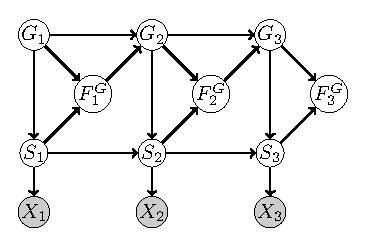
\epsfig{file=fig/ahmm.eps}
\caption{Dynamic Bayesian network representation of 1-level AHMM~\cite{murphy02}.}
\label{fig:ahmm}
\end{figure}

One difference between this 1-level AHMM and a general HHMM is that state $S_t$ never
``resets'', since $F^G_t$ is not a parent. Here we assume that during a gesture sequence, even if the goal changes,
the next state of the hand/arm movement always depends on the previous state. This is reasonable for gesture recognition because the hand/arm 
movement is always continuous (unless the hands move out of the sensor's view during
which the inference engine will reset). 

Let $Z_t = (G_t, S_t, F^G_t, X_t)$. The joint distribution of the sequence $Z_1, \ldots, Z_T$
is
\begin{displaymath}
P(Z_{1:T}) = \prod_{t = 1}^{t = T}\prod_{i = 1}^{4}P(Z_t^i|Pa(Z_t^i))
\end{displaymath}
where $Z_t^i$ is the $i$'th node at time $t$, and $Pa(Z_t^i)$ are the parents. 
$P(Z_t^i|Pa(Z_t^i))$ are defined by a set of conditional probability distributions (CPD) which
includes
\begin{align}
P(G_1 = i) &= \text{prior for } G \label{eq:cpd-g1} \\ 
P(S_1 = j | G_1 = i) &= \text{prior for } S \\
P(G_t = j| G_{t - 1} = i, F_{t - 1}^G = f) &= 
\begin{cases}
  \delta(i, j), & \text{if} f = 0 \\
  A^G(i, j), & \text{if} f = 1 
\end{cases} \label{eq:cpd-g2}\\
P(F_t^G = 1 | G_t = g, S_t = i) &= A_g^S(i, \text{end}) \\
P(S_t = j | G_{t - 1} = g, S_{t - 1} = i) &= A_g^S(i, j) \label{eq:cpd-s}\\
P(X_t = x_t | S_t = i) &= N(x_t; \mu_i, \Sigma_i). \label{eq:cpd-x}
\end{align}
Here, $\delta(i, j) = 1$ if $i == j$ and $0$ otherwise, and $A^Q_q(i, j)$ is the
transition probability for node $Q$ from state $i$ to $j$ when its parent is $q$.
Since $G_t$, $S_t$ and $F_t$ take discrete values, CPD(\ref{eq:cpd-g1})-(\ref{eq:cpd-s})
can be represented in table forms. $X_t$ is a continuous vector and CPD(\ref{eq:cpd-x})
is a Gaussian distribution.

We use the 2TBN-based (2-slice temporal Bayes net)
junction tree algorithm as the lower level inference engine\footnote{\url{http://bnt.googlecode.com/svn/trunk/docs/usage_dbn.html}}  
and use forward/backward operators on top of that to do exact inference on the graph.

\subsection{Hand Feature}
We combine both hand motion features, $X^M_t$ and hand pose features, $X^P_t$
for the observed feature vector $X_t$, i.e., 
\begin{displaymath}
X_t = \left[ \begin{array}{c}
X^M_t\\
X^P_t
\end{array}\right]
\end{displaymath} 

The motion features include the relative position ($\bf{p}$), velocity ($\bf{v}$),
and acceleration ($\bf{a}$) of the center of
the hand bounding box.
All of them are 3-dimensional vectors in the world
coordinate system, hence $X_t^M\in\mathbb{R}^9$. 

The hand pose features are computed from a $100 \times 100$ px image $I_{h}$ scaled
from the bounding box of the final tracked hand (Figure~\ref{fig:depth}). Each pixel
is a depth value scaled between $0$ and $255$. We explore several hand pose 
features derived from $I_h$.

\begin{figure}
\centering
\begin{subfigure}{1\columnwidth}
\includegraphics[width=1\columnwidth]{fig/hand-depth.ps}
\caption{Depth images, $I_h$}
\label{fig:depth}
\end{subfigure}
\begin{subfigure}{1\columnwidth}
\includegraphics[width=1\columnwidth]{fig/hand-hog.ps}
\caption{HOG descriptor with $sBin = 8$ and $oBin = 9$}
\label{fig:hog}
\end{subfigure}
\begin{subfigure}{1\columnwidth}
\includegraphics[width=1\columnwidth]{fig/hand-hog-30-36.ps}
\caption{HOG descriptor with $sBin = 30$ and $oBin = 36$}
\label{fig:hog-30}
\end{subfigure}
\caption{Visualization hand image and hand pose features.}
\label{fig:hand-vis}
\end{figure}

\subsubsection{Eigenhand}\label{sec:eigenhand}
This is similar to the eigenface~\cite{turk91} technique. We concatenate the
rows of the hand image, $I_h$, into a column vector and perform principle
component analysis (PCA) on all the training images. The images
reshaped from the eigenvectors are the eigenhands. We use
the first $d$ eigenvectors, $u_1, \ldots, u_d$, corresponding to the 
$d$ largest eigenvalues as our basis.
Hence, the hand pose feature vector, $X_t^P$ is a $d$-dimensional vector $[w_1,
\ldots, w_d]$ where each component is the projection of the hand into each
eigenvectors $u_1, \ldots, u_d$.

\subsubsection{HOG}\label{sec:hog}
The original HOG descriptor for pedestrian detection is based on RGB images. As
a result local contrast normalization is important for better invariance to
illumination~\cite{dalal05}. In their evaluation, a 4-fold normalization
gives the best performance. Our hand images are based on depth values, and are less
affected by illumination variation. Hence, we only use the descriptor from the first fold
out of the 4-fold normalization. Different spatial bin (cell) size, $sBin$, and
different number of orientation bins, $oBin$, may be used. Figure~\ref{fig:hog}
shows the visualization of HOG descriptors for several example $I_h$.
In particular, the feature used by Freeman and Roth can be viewed 
as a special case of HOG with 1 spatial bin and 36 orientation bins (Figure~\ref{fig:hog-30}).

With a small spatial bin size, the size of the HOG descriptor for a $100\times 100$ px image can be
quite large. For example, when $sBin = 8$, and $oBin = 9$, the length of HOG using 1 out of 4-fold
normalization is $(100/8 - 2)^2\times 9 = 900$. Hence, we use PCA to reduce the dimension to $n$.
In object recognition, using PCA to do dimensionality reduction often results in less
favorable results. Hariharan et al.~\cite{Hariharan12} show that this is because the dimensions of the most variation retained by 
PCA often correspond to variation in illumination and viewing direction, and the dimensions
that are ignored are often those that are the most discriminative. These arguments may not
be applicable in our case because: (1) our images are based on depth values and hence are less
susceptible to illumination variation; (2) we want to distinguish different hand shapes instead of grouping hands with different poses
together. Thus, looking at the dimensions with the largest variation may be useful.

We compare the gesture recognition results using different hand pose features with different parameters in Section~\ref{sec:eval}.

\subsection{Learning}
We use supervised training to learn the parameters (i.e., CPDs) of the 1-level AHMM DBN model.
The training data has $G_t$, $F_t^G$ and $X_t$ observed, but $S_t$ is hidden.
Since the data is partially observed, we use expectation maximization (EM)
algorithms to learn the maximum likelihood estimate of the parameters. 

The result of EM depends on good initialization. As we model the production probability $P(X_t | S_t)$ as a Gaussian distribution, we
can view $X_t$ as a mixture of Gaussians. The number of states $S_t$ can take is the
number of mixtures (i.e., clusters). In addition, for dynamic hand poses, there is no
distinct classes of hand shapes. As a result, we use unsupervised clustering analysis of the training data and
using the Bayesian information criterion (BIC)~\cite{fraley12} to find the optimal number of clusters. 
Then we set the number of state for $S_t$
to be the number of clusters, and initialize $\mu_i$ to be the cluster centers. 
We also use clustering analysis to determine the optimal number of PCA components $d$ to use.

\subsection{Inference}
There are different kinds of inference one can perform on a DBN. For online gesture
recognition, to make the system the most responsive, we need to do \textit{online filtering} which is to recursively estimate the
belief state~\cite{murphy02} using the forward algorithm and find the optimal gesture phase
at time $t$ as:
\begin{displaymath}
g^* = \arg\max_g P(G_t = g | x_{1:t}) 
\end{displaymath}

However, there can be a trade-off between responsiveness and accuracy. If we allow some lag $L$,
we can use more evidence to estimate the gesture phase of past at $t - L$ as:
\begin{align*}
g^* = \arg\max_g P(G_{t - L} = g | x_{1 : t} )
\end{align*}
This is traditionally called ``\textit{fixed-lag smoothing}'' and can often give higher
accuracy. Online filtering is a special case when $L = 0$.

The other extreme is the offline case, where the whole sequence of length $T$ is known. In this case
we can compute the optimal gesture phase for each time frame $t$ as:
\begin{align*}
g^* = \arg\max_g P(G_t = g | x_{1 : T}).
\end{align*}
This is also called ``\textit{fixed-interval smoothing}'' and should give an 
upper bound in gesture recognition for the model.

Given the frame rate and human reaction time, we can allow a few frames of lag in order
to achieve better accuracy without substantial reduction in the utility of the system. 
Section~\ref{sec:comp-inf} shows the experimental comparison of different
inference methods.

\section{Experimental Evaluation}\label{sec:eval}
We conduct user-dependent evaluation of our hand tracking and gesture recognition algorithm based on
a publically available corpus.

\subsection{Data set}
We use part of the ChAirGest corpus~\cite{Ruffieux2013} as our data set. There are 10 gestures (Table~\ref{tab:gesture}) and
3 resting postures (hands on then table, hands on the belly , and hands under the chin) in the corpus. Each gesture consists
pre-stroke, gesture nucleus and post-stroke~\cite{Pavlovic97}. Only the left hand is used
in all the gestures. 

\begin{table}[tb]
\begin{center}
\caption{Gestures in the corpus and their hand poses. }
\label{tab:gesture}
\begin{tabular}{|l|l|}
\hline
\textbf{\# and Name of gestures} & \textbf{Hand pose} \\
\hline
1 Shake hand & Static \\
\hline
2 Wave hello & Static\\
\hline
3 Swipe right & Static \\
\hline
4 Swipe left &  Static \\
\hline
\multicolumn{1}{|p{0.38\columnwidth}|}{5 Draw a circle with rotating palm} & Dynamic\\
\hline
\multicolumn{1}{|p{0.38\columnwidth}|}{6 Draw a circle with palm down} & Static \\
\hline
7 Take from screen & Dynamic (grab motion) \\
\hline
8 Push to screen & Static \\
\hline
9 Palm-down rotation & Dynamic (rotating palm)\\
\hline
10 Palm-up rotation & Dynamic (rotating palm) \\
\hline
\end{tabular}
\end{center}
\end{table}

We use recordings from 4 participants, and for each participant, we use 2 sessions of recordings.     
In each session, there are 7-8 sequences with 2-5 gesture occurrences 
sequence. Overall there are 2 occurrence for each gesture/resting posture combination per subject. 

\subsection{Method}
For each participant, we use
one tenth of the sequences for testing and the remaining for training. The RGB and depth videos are 30 fps (frame per second) and we down-sample them
to 10 fps to increase the training speed. This results in about 600 frames per sequence on average.

We treat the preparation phase (\#11), the retraction phase (\#12) and the rest posture (\#13) as different gesture classes, resulting
in 13 gesture classes. In this data set, all gesture occurrences follow the pattern: rest $\rightarrow$ preparation
$\rightarrow$ gesture nucleus $\rightarrow$ retraction $\rightarrow$ rest and then repeat. 
Hence, we initialize the prior distribution CPD (Eqn~(\ref{eq:cpd-g1}))
and the transition probability CPD (Eqn~(\ref{eq:cpd-g2})) for $G$ such that the probability of transition from the preparation phase
to one of the ten gesture nucleus phases is uniform and all other transitions are deterministic.

We use data from one training session of one participant to do mixture of Gaussian
clustering analysis\footnote{\url{http://cran.r-project.org/web/packages/mclust/index.html}} using Eigenhand feature for $X_t^P$. 
Our results show that $36$ clusters and
$7$ PCA components (Figire~\ref{fig:bic}) give the highest BIC. Hence we set the number of hidden states $S_t$ to be $36$ and $d = 7$
in the PCA dimensionality reduction of the hand pose feature $X_t^P$.

\begin{figure}
\centering
\includegraphics[width=1\columnwidth]{fig/loglik-feature-1.ps}
\caption{Plot of loglikelihood (red) and BIC (blue) of Gaussian mixture models with different
number of features for $X_t$. The number of clusters is $36$. BIC adds regularization to the 
complexity of the model, and is the highest when the number of features
is 16. As the 9-dimensional motion feature $X_t^M$ is always included, the optimal value for $d$ is $7$ in the PCA reduction 
of the hand pose feature $X_t^P$.}
\label{fig:bic}
\end{figure}

To compare recognition performance, we compute frame-based accuracy and F1 score. 
A frame is considered correctly classified if its predicted label is equal to the ground truth label.
Hence frame accuracy is computed as
\begin{displaymath}
\text{frame accuracy} = \frac{\text{\# correctly classified frames}}{\text{\# frames in the sequence}}
\end{displaymath}
Because we have a multi-class classification problem, we compute F1 score for each gesture class and 
the overall F1 score is the average from all gesture classes.

We used the Bayes Net Toolbox for Matlab\footnote{\url{https://code.google.com/p/bnt/}} to implement the training
and inference of the AHMM DBN.

\subsection{Hand Pose Feature Comparison}
Table~\ref{tab:comp-feature} shows the comparison of the recognition performance with different hand pose features $X_t^P$. The 
hand motion feature $X_t^M$ is kept the same. All results are based on fixed-interval smoothing inference.
Note that $n$ is the number of PCA components mentioned in Section~\ref{sec:eigenhand} and $sBin$ is the
cell size and $oBin$ is the number of orientation bins mentioned in Section~\ref{sec:hog}.

The results show that using HOG descriptor with cell size = 4px and 9 orientation bins
gives the best recognition performance. This cell size is smaller than what is commonly used for 
pedestrian detection~\cite{dalal05}, possibly because the fingers are thinner than
body limbs and hence finer spatial binning is helpful.

\begin{table}[tb]
\begin{center}
\caption{Per frame gesture classification accuracy and F1 scores in \% for different
hand pose features on the test data set. The results are the average from all test
sequences from 4 participants. Numbers in parentheses are standard deviations.}
\label{tab:comp-feature}
\begin{tabular}{|l|c|c|}
\hline
\textbf{Hand pose feature} & \textbf{Accuracy} & \textbf{F1} \\
\hline
Eigenhand (d = 7) & 83.3 (4) & 74.8 (8) \\ 
\hline
HOG (sBin = 4, oBin = 9, d = 7) & 84.0 (3) & 79.7 (8)\\
\hline
HOG (sBin = 8, oBin = 9, d = 7) & 84.0 (3) & 74.6 (2)\\
\hline
HOG (sBin = 30, oBin = 12, d = 7) & 70.9 (6) & 70.9 (9)\\
\hline
\end{tabular}
\end{center}
\end{table}

\subsection{Inference temporal lag comparison} \label{sec:comp-inf}
Using the HOG descriptor ($sBin = 8$ and $oBin = 9$) followed by PCA dimensionality
reduction to $d = 7$ PCA components for hand pose features, we compare the frame-based
classification result for different inference methods. Table~\ref{tab:comp-inf}
shows that online filtering gives the lowest frame classification accuracy and F1 score as
expected. However, once we add a lag of 16 frames, the F1 score increases to 72.3\%,
a 38\% improvement. 
 
Figure~\ref{fig:comp-inf}
further illustrates the promising result that a small time lag in estimating the 
gesture phase can result in a large improvement in accuracy. With a frame rate of 30fps, 16 frames is about 0.5s. 

\begin{table}[tb]
\begin{center}
\caption{Comparison of frame-based classification performance with different temporal lag.}
\label{tab:comp-inf}
\begin{tabular}{|l|c|c|}
\hline
\textbf{Temporal lag} & \textbf{Accuracy} & \textbf{F1}  \\
\hline
Online filtering (L = 0) & 73.8 (4) & 52.3 (6)\\
\hline
Fixed-lag smoothing (L = 1) & 79.2 (3) & 55.7 (7)  \\
\hline
Fixed-lag smoothing (L = 2) & 80.2 (3) & 58.6 (7) \\
\hline
Fixed-lag smoothing (L = 4) & 81.6 (3) & 64.6 (5) \\
\hline
Fixed-lag smoothing (L = 8) & 83.5 (3) & 69.5 (5) \\
\hline
Fixed-lag smoothing (L = 16) & 83.8 (3) & 72.3 (3) \\
\hline
Fixed-interval smoothing & 84.0 (3) & 74.6 (2)\\ 
\hline
\end{tabular}
\end{center}
\end{table}

\begin{figure}
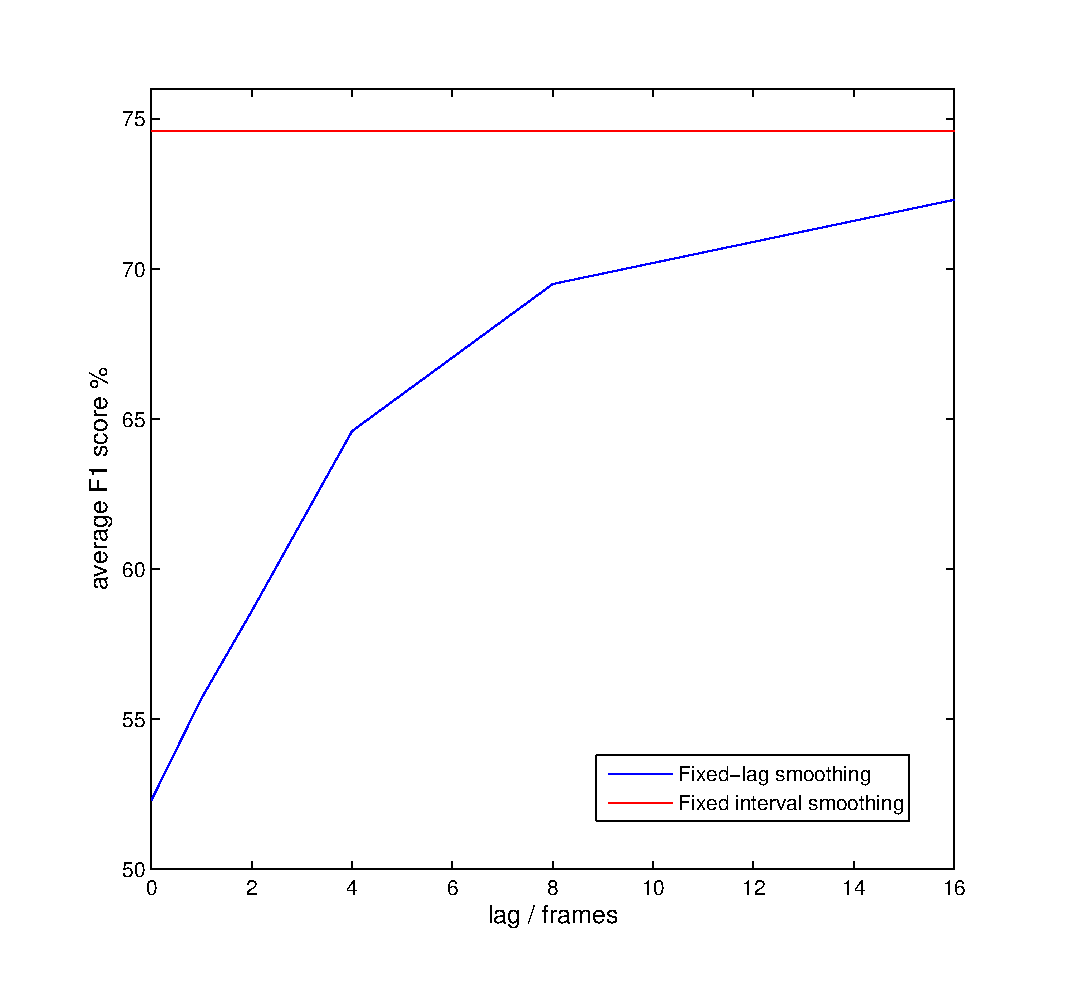
\epsfig{file=fig/f1-lag.eps, width=1\columnwidth}
\caption{Plot of average F1 score \% against frame
   lag in online inference. The red line is the result from fixed-interval
   smoothing which is an upper bound for the recognition performance.}
\label{fig:comp-inf}
\end{figure}

\subsection{Gesture classification confusion matrix}
Using fixed-interval smoothing inference and the same hand pose feature in the previous
section, we compute the frame-based confusion matrix
between the ground truth gesture labels and the predicted ones. Figure~\ref{fig:confusion-matrix} shows that most gesture phase classification errors
occur between the preparation (\#11) phase / the retraction (\#12) phase and the other gesture nucleus phases. We
observe that the transitions between these phases are usually
not very clear even to the human eyes, and hence accurate detection of the boundaries between these
phases can be hard. For many applications, the accurate detection of the boundaries may not be
necessary either.

\begin{figure}
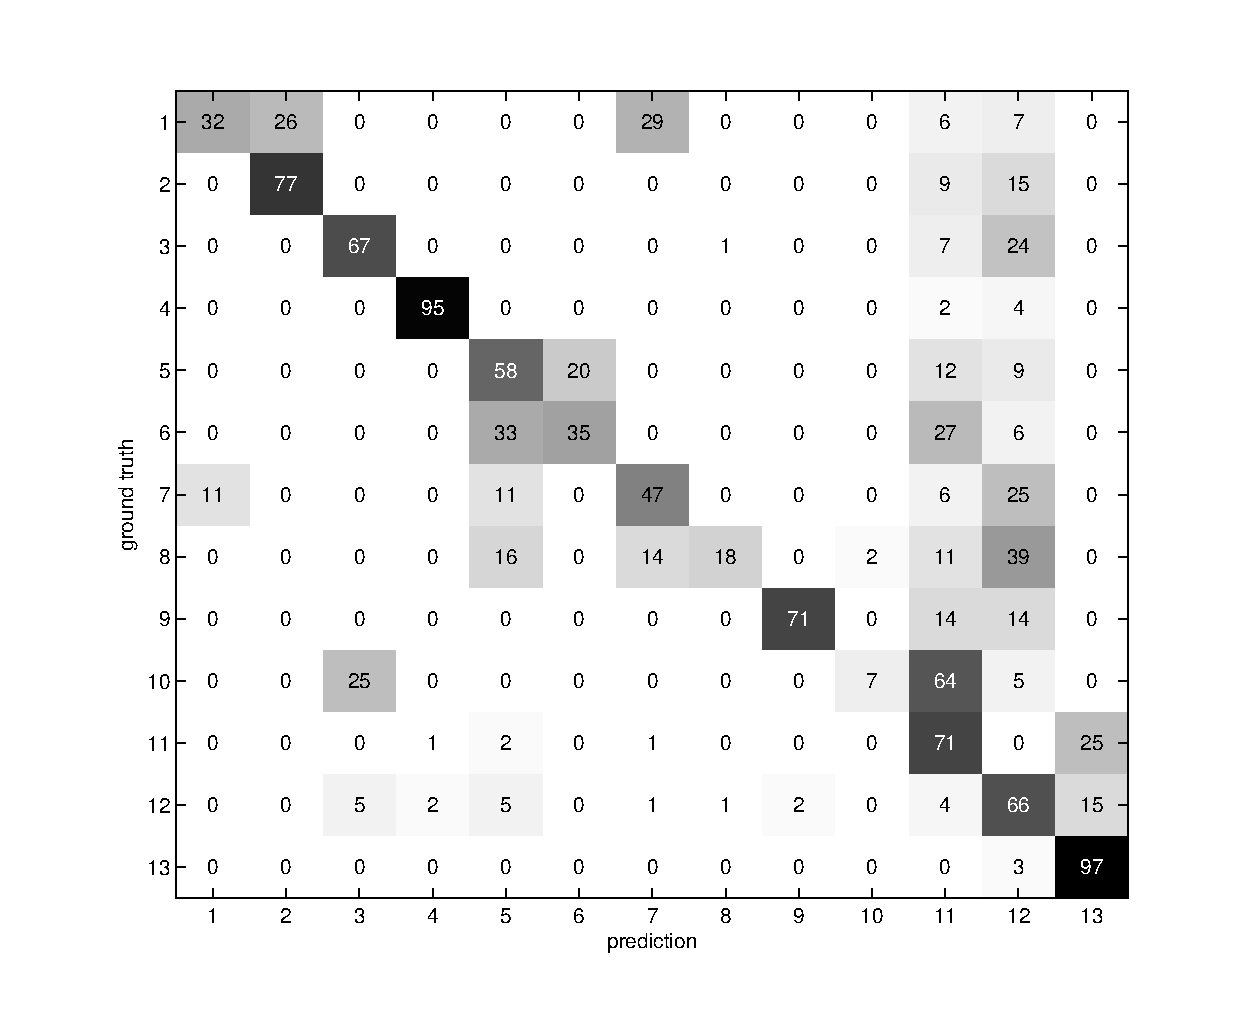
\includegraphics[width=1.1\columnwidth]{fig/confusion-matrix.eps}
\caption{Confusion matrix of ground truth gesture labels vs.
   predicted gesture labels for each frame. }
\label{fig:confusion-matrix}
\end{figure}

We also note that this data set has a few gestures that are particularly hard to recognize.
For example the ``Palm-up rotation'' gesture (\#10) is similar to the ``Swipe right'' gesture (\#3) as they 
have the same motion trajectory. The difference is that the hand rotates in the ``Palm-up rotation'' gesture whereas the 
hand stays the same in the ``Swipe right'' gesture. However, some participants rotate their hands when doing
the ``Swipe right'' gesture as well (see Figure~\ref{fig:swipe-right}).

\begin{figure}
\centering
\begin{subfigure}{1\columnwidth}
\includegraphics[width=1\columnwidth]{fig/swipe-right-correct.ps}
\caption{Correct Swipe-right gesture.}
\label{fig:depth}
\end{subfigure}
\begin{subfigure}{1\columnwidth}
\includegraphics[width=1\columnwidth]{fig/swipe-right-wrong.ps}
\caption{Incorrect Swipe-right gesture where the participant rotates the palm making it
the same as Palm-up rotation gesture.}
\label{fig:hog}
\end{subfigure}
\caption{Examples of participants doing the gestures.}
\label{fig:swipe-right}
\end{figure}


\section{Future Work}
We note that our method of combining skin color detection, user detection and
skeleton tracking can fail when the user is wearing clothes with color similar
to the skin color. Using a probability distribution of skin color instead
of binary classification can be more robust. We also want to experiment with using STIP (spatial temporal
interest points) feature~\cite{laptev2003} to improve hand tracking or using it as hand pose feature.

As we derive hand features from tracked hand images, the recognition performance is
highly dependent on accurate hand tracking. Any ill condition can lead to degraded performance. 
As body tracking can be relatively more robust than hand tracking, we also want to experiment with
using features such as HOG and STIP descriptors derived from body image as input to
the AHMM gesture recognition framework. 

We will also consider two-hand gestures in future work, perhaps by tracking both hands
as we tracked one hand here, or by using features derived from body images directly which would incorporate both hands as well. 

\section{Conclusions}
Our evaluation show that the HOG descriptor and PCA dimensionality reduction
can be effective for recognition of gestures with dynamic hand pose and path. In particular, 
a spatial binning for the HOG descriptor finer than used traditionally gives a better recognition result. 
Our AHMM-based gesture recognition framework can incorporate hand pose features in the Gaussian CPD of
the observation node. 

The AHMM models the gesture segmentation and gesture transition directly by using the termination
indicator node $F_t$. It incorporates both the segmentation and gesture recognition together
during the probabilistic inference, making it easier to implement than the mixture of flat HMMs when handling
continuous gesture recognition with unsegmented and unbounded input.  

We can perform online inference with different time lag, making trade-off between accuracy and responsiveness depending on the 
application requirement. In particular, a delay in about 16 frames (0.5s) can improve the recognition performance by
38\%, making it close to off-line performance.
 
%\end{document}  % This is where a 'short' article might terminate

%ACKNOWLEDGMENTS are optional
\section{Acknowledgments}
We would like to thank our lab mate for providing the initial implementation of 
the experiment framework in MATLAB for running training and testing tasks in parallel.

% The following two commands are all you need in the
% initial runs of your .tex file to
% produce the bibliography for the citations in your paper.
\bibliographystyle{abbrv}
\bibliography{sigproc}  % sigproc.bib is the name of the Bibliography in this case
% You must have a proper ".bib" file
%  and remember to run:
% latex bibtex latex latex
% to resolve all references
%

\balancecolumns % GM June 2007
% That's all folks!
\end{document}
